% Provenance (never printed): cycle 4 SVT, "La planete Terre": the dynamics of
% the Earth's outer shell, plates and their boundaries, continental drift as a
% history of ideas; see sources/outline_sources.md. Pilot chapter, 2026-10-22.
\chapter{Plate Tectonics: The Moving Puzzle}\label{ch:g7:plate-tectonics}

Spread a \omterm{def:g2:drawing-to-map:map}{map} of the world on a table and look at the two shores of the
Atlantic \omterm{def:g2:water-on-earth:ocean}{Ocean}. The great bulge of Brazil seems made to slide into the
hollow of Africa's west \omterm{def:g1:landscapes-around-us:water}{coast}, as if someone had cut a single piece of
land in two and pushed the halves apart. The first people to print good
\omterm{def:g2:drawing-to-map:map}{maps} of both \omterm{def:g1:landscapes-around-us:water}{coasts} noticed it at once. For three centuries it remained a
curiosity. In the twentieth century it became the starting point of the
theory that now explains why the ground shakes in Japan, why the Andes are
so high, why Iceland is slowly growing wider --- and why the \omterm{def:g2:drawing-to-map:map}{map} on the
table is only a snapshot of a world that is moving.

\begin{omfigure}
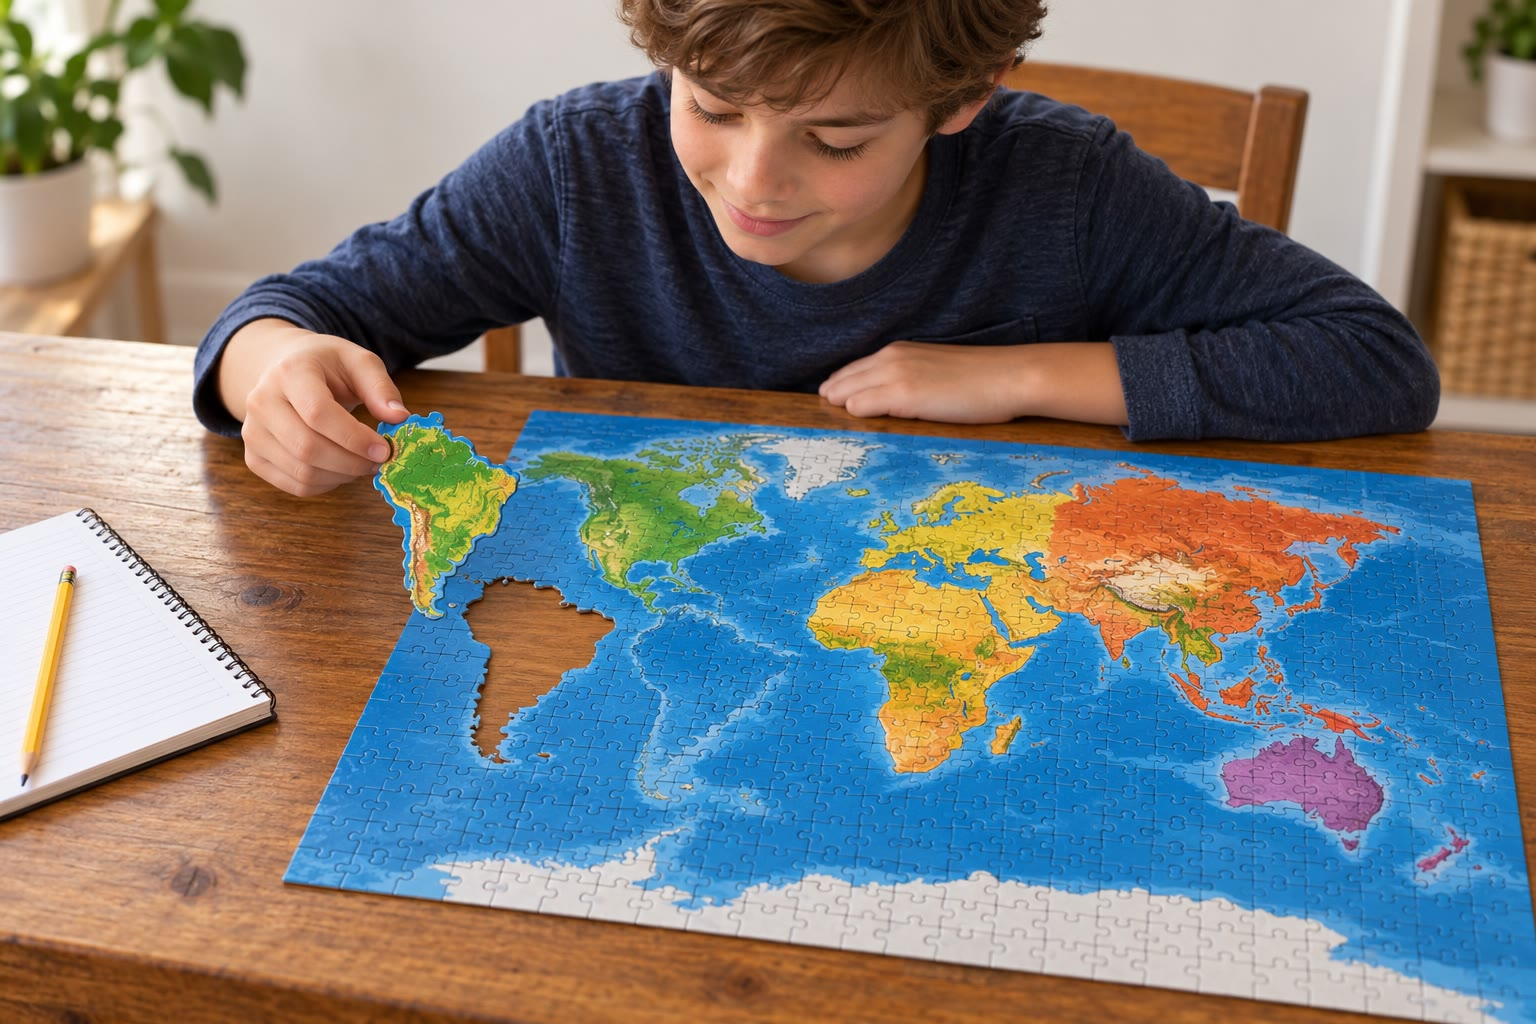
\includegraphics[width=0.62\linewidth]{images/book1/ai/g7-puzzle-map.jpg}

{\small South America next to Africa: on a puzzle, the fit is a game; on
the real Earth, it is a clue.}
\end{omfigure}

\begin{recall}
The Earth has three main layers: a thin, rocky \emph{\omterm{def:g6:inside-the-earth:layers}{crust}}, a thick
\emph{\omterm{def:g6:inside-the-earth:layers}{mantle}} of hot \omterm{def:g3:stones-pebbles-sand:rock}{rock}, and a metallic \emph{\omterm{def:g6:inside-the-earth:layers}{core}}; temperature rises
with depth (\cref{ch:g6:inside-the-earth}). A place on the \omterm{def:g3:continents-and-oceans:globe}{globe} is located
by its \omterm{def:g6:latitude-longitude:latitude}{latitude} and its \omterm{def:g6:latitude-longitude:longitude}{longitude} (\cref{ch:g6:latitude-longitude}).
\end{recall}

\section{Continents that once fitted together}

\begin{definition}[Continental drift]\label{def:g7:plate-tectonics:continental-drift}
\emph{Continental drift}\index{continental drift} is the idea that the
\omterm{def:g3:continents-and-oceans:continent}{continents} move slowly across the surface of the Earth, so that their
positions, and the shapes of the \omterm{def:g2:water-on-earth:ocean}{oceans} between them, have changed over
the ages.
\end{definition}

\begin{definition}[Supercontinent]\label{def:g7:plate-tectonics:supercontinent}
A \emph{supercontinent}\index{supercontinent} is a single landmass made of
all, or almost all, of the \omterm{def:g3:continents-and-oceans:continent}{continents} joined together. The last one,
\emph{Pangaea}\index{Pangaea} (``all lands'' in Greek), began to break up
between about 225 and 200 million years ago.
% ledger: usgs:pangaea-breakup
\end{definition}

The scientist who defended \omterm{def:g7:plate-tectonics:continental-drift}{continental drift} as a real theory, with
evidence, was Alfred Wegener. He gathered four kinds of clues.

\begin{enumerate}
  \item \textbf{The shapes of the \omterm{def:g1:landscapes-around-us:water}{coasts}.} South America and Africa fit
        together like two pieces of a jigsaw, and so do several other
        coastlines.
  \item \textbf{Fossils.} The same fossil animals and plants are found on
        \omterm{def:g3:continents-and-oceans:continent}{continents} that are now separated by thousands of kilometres of
        \omterm{def:g2:water-on-earth:ocean}{ocean}. \emph{Mesosaurus} was a small reptile that lived in \omterm{def:g2:water-on-earth:salt-fresh}{fresh
        water}: it could not have swum across an \omterm{def:g2:water-on-earth:ocean}{ocean}, yet its fossils lie
        both in Brazil and in southern Africa.
  \item \textbf{\omterm{def:g3:stones-pebbles-sand:rock}{Rocks}.} \omterm{def:g3:stones-pebbles-sand:rock}{Rocks} of the same kinds and ages, and old \omterm{def:g1:landscapes-around-us:landform}{mountain}
        chains of the same shape, stop at one \omterm{def:g1:landscapes-around-us:water}{coast} and start again on the
        opposite one, as the lines of print on a torn newspaper do.
  \item \textbf{Ancient \omterm{def:g5:weather-and-climate:climate}{climates}.} Coal, made from the plants of warm,
        swampy forests, is found in Antarctica; traces left by ancient
        glaciers are found in parts of Africa that are now hot and dry.
        These lands must once have lain in other \omterm{def:g5:weather-and-climate:climate}{climates}, at other
        \omterm{def:g6:latitude-longitude:latitude}{latitudes}.
\end{enumerate}
% ledger: usgs:coal-antarctica, usgs:fossil-map

\begin{omfigure}
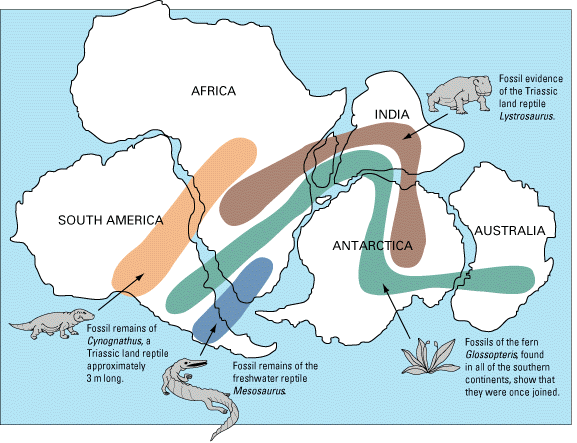
\includegraphics[width=0.86\linewidth]{images/book1/g7-usgs-fossil-map.png}

{\small The southern \omterm{def:g3:continents-and-oceans:continent}{continents} put back together. Each coloured band joins
the places where one fossil species is found today: the land reptiles
\emph{Cynognathus} and \emph{Lystrosaurus}, the freshwater reptile
\emph{Mesosaurus} and the fern \emph{Glossopteris}. Separated, the
\omterm{def:g3:continents-and-oceans:continent}{continents} scatter the bands; joined, the bands run on without a break.
\omterm{def:g2:drawing-to-map:map}{Map}: U.S. Geological Survey, \emph{This Dynamic Earth} (public domain).}
\end{omfigure}

\begin{history}[Wegener's idea, 1912--1930]
% ledger: usgs:wegener-1912, usgs:wegener-death, usgs:jeffreys
Alfred Wegener, a 32-year-old German meteorologist, set out the theory of
\omterm{def:g7:plate-tectonics:continental-drift}{continental drift} in two articles in 1912. Most geologists rejected it.
The strongest objection was that Wegener could not say \emph{what} moved
the \omterm{def:g3:continents-and-oceans:continent}{continents}: he thought they ploughed through the \omterm{def:g3:stones-pebbles-sand:rock}{rock} of the \omterm{def:g2:water-on-earth:ocean}{ocean}
floor, and the physicist Harold Jeffreys showed that solid \omterm{def:g3:continents-and-oceans:continent}{continents} could
not do that without breaking up. Wegener went on collecting evidence until
he died on the Greenland ice cap in 1930, during an expedition. The answer
he lacked came from the floor of the \omterm{def:g2:water-on-earth:ocean}{oceans}, explored after the 1950s: it
is told in a later year.
\end{history}

\section{The plates}

Wegener's clues were right, but his \omterm{def:g3:continents-and-oceans:continent}{continents} were the wrong pieces. It is
not only the \omterm{def:g3:continents-and-oceans:continent}{continents} that move: the whole outer shell of the Earth,
under the \omterm{def:g3:continents-and-oceans:continent}{continents} and under the \omterm{def:g2:water-on-earth:ocean}{oceans} alike, is broken into pieces.

\begin{definition}[Tectonic plate]\label{def:g7:plate-tectonics:plate}
A \emph{tectonic plate}\index{tectonic plate} (or simply a plate) is a
large, rigid slab of \omterm{def:g3:stones-pebbles-sand:rock}{rock} that forms part of the Earth's outer shell. A
plate is made of the \omterm{def:g6:inside-the-earth:layers}{crust} and of the uppermost, cold and rigid part of the
\omterm{def:g6:inside-the-earth:layers}{mantle}, together at least 80 kilometres thick on average; it moves slowly
over the hotter and softer \omterm{def:g6:inside-the-earth:layers}{mantle} beneath it.
% ledger: usgs:lithosphere-80km
\end{definition}

\begin{definition}[Plate tectonics]\label{def:g7:plate-tectonics:plate-tectonics}
\emph{Plate tectonics}\index{plate tectonics} is the theory that the outer
shell of the Earth is divided into \omterm{def:g7:plate-tectonics:plate}{plates} that move relative to one
another, and that most \omterm{def:g4:volcanoes-earthquakes-first-look:earthquake}{earthquakes}, \omterm{def:g4:volcanoes-earthquakes-first-look:volcano}{volcanoes} and \omterm{def:g4:world-physical-map:range}{mountain ranges} are
produced where \omterm{def:g7:plate-tectonics:plate}{plates} meet.
\end{definition}

\begin{remark}[How many plates?]\label{rem:g7:plate-tectonics:how-many}
% ledger: usgs:plates-dozen, pb2002:count
About a dozen \omterm{def:g7:plate-tectonics:plate}{plates} are large; many more are small. A detailed \omterm{def:g2:drawing-to-map:map}{map} used by
geologists counts 52 of them. A \omterm{def:g7:plate-tectonics:plate}{plate} may carry a \omterm{def:g3:continents-and-oceans:continent}{continent}, an \omterm{def:g2:water-on-earth:ocean}{ocean}, or
both: the South American \omterm{def:g7:plate-tectonics:plate}{plate} carries the whole of South America and the
western half of the South Atlantic \omterm{def:g2:water-on-earth:ocean}{Ocean}. The Pacific \omterm{def:g7:plate-tectonics:plate}{plate}, the largest,
carries almost no land at all.
\end{remark}

\begin{omfigure}
\begin{tikzpicture}
\begin{axis}[ommap, width=\linewidth, xtick={-180,-90,...,180}, ytick={-60,0,60}]
\addplot[fill=omLithAlluv, draw=black!45, line width=0.2pt] table {figdata/out/shared-geo-land.dat};
\addplot[omRidge, line width=0.8pt] table {figdata/out/shared-geo-school-ridge.dat};
\addplot[omRidge!70!black, line width=0.8pt] table {figdata/out/shared-geo-school-transform.dat};
\addplot[omTrench, line width=0.8pt] table {figdata/out/shared-geo-school-subduction.dat};
\addplot[fill=omTrench, draw=none] table {figdata/out/shared-geo-school-teeth.dat};
\addplot[black!65, line width=0.8pt] table {figdata/out/shared-geo-school-collision.dat};
\begin{scope}[every node/.style={font=\scriptsize\bfseries, text=black!85,
    fill=white, fill opacity=0.75, text opacity=1, inner sep=1pt, align=center}]
  \node at (axis cs:-150,12) {Pacific};
  \node at (axis cs:-103,52) {North\\American};
  \node at (axis cs:-48,-12) {South\\American};
  \node at (axis cs:85,57) {Eurasian};
  \node at (axis cs:18,8) {African};
  \node at (axis cs:10,-75) {Antarctic};
  \node at (axis cs:78,11) {Indian};
  \node at (axis cs:128,-26) {Australian};
  \node at (axis cs:-95,-22) {Nazca};
  \node at (axis cs:50,20) {Arabian};
\end{scope}
\end{axis}
\end{tikzpicture}

{\small The main \omterm{def:g7:plate-tectonics:plate}{tectonic plates}. Red: \omterm{def:g7:plate-tectonics:plate}{plates} moving apart; blue with
triangles: one \omterm{def:g7:plate-tectonics:plate}{plate} sinking under the other (the triangles are on the
\omterm{def:g7:plate-tectonics:plate}{plate} that stays on top); grey: \omterm{def:g7:plate-tectonics:plate}{plates} pushing together across a wide zone
of \omterm{def:g1:landscapes-around-us:landform}{mountains}; dark red: \omterm{def:g7:plate-tectonics:plate}{plates} sliding past each other. Boundaries after
P.~Bird (2003); coastlines from Natural Earth.}
\end{omfigure}

How do we know where one \omterm{def:g7:plate-tectonics:plate}{plate} ends and the next begins? Look at where the
Earth is restless.

\begin{proposition}[Earthquakes and volcanoes trace the plate boundaries]\label{prop:g7:plate-tectonics:restless}
% ledger: data:usgs-comcat, data:pb2002 (share computed in figdata/grade-7/quakes_on_boundaries.py)
\omterm{def:g4:volcanoes-earthquakes-first-look:earthquake}{Earthquakes} and \omterm{def:g4:volcanoes-earthquakes-first-look:volcano}{volcanoes} are not scattered at random over the Earth: most
of them lie along narrow belts, and these belts are the edges of the
\omterm{def:g7:plate-tectonics:plate}{plates}. Of the 7\,031 \omterm{def:g4:volcanoes-earthquakes-first-look:earthquake}{earthquakes} of magnitude 6 or more recorded between
1976 and 2025, 6\,472 --- that is 92\,\% --- happened less than
\qty{300}{km} from a \omterm{def:g7:plate-tectonics:plate-boundary}{plate boundary}.
\end{proposition}

\begin{omfigure}
\begin{tikzpicture}
\begin{axis}[ommap, width=\linewidth, xtick={-180,-90,...,180}, ytick={-60,0,60},
  legend style={at={(0.02,0.04)}, anchor=south west, font=\scriptsize,
  fill=white, fill opacity=0.85, text opacity=1, draw=black!40}]
\addplot[fill=omLithAlluv, draw=black!45, line width=0.2pt, forget plot] table {figdata/out/shared-geo-land.dat};
\addplot[only marks, mark=*, mark size=0.45pt, omThm!85!black] table[x=lon, y=lat] {figdata/out/grade-7-quakes_on_boundaries-map.dat};
\addlegendentry{earthquake, magnitude 6.5 or more, 1976--2025}
\addplot[only marks, mark=triangle*, mark size=1.1pt, black] table {figdata/out/shared-geo-volcanoes.dat};
\addlegendentry{volcano active in the last 12\,000 years}
\end{axis}
\end{tikzpicture}

{\small Large \omterm{def:g4:volcanoes-earthquakes-first-look:earthquake}{earthquakes} and recent \omterm{def:g4:volcanoes-earthquakes-first-look:volcano}{volcanoes}. Compare with the \omterm{def:g2:drawing-to-map:map}{map} of the
\omterm{def:g7:plate-tectonics:plate}{plates} above: the dots and the triangles draw the \omterm{def:g7:plate-tectonics:plate-boundary}{plate boundaries}. Data:
U.S. Geological Survey \omterm{def:g4:volcanoes-earthquakes-first-look:earthquake}{earthquake} catalogue; Smithsonian Global Volcanism
Program.}
\end{omfigure}

\section{Three kinds of plate boundaries}

\begin{definition}[Plate boundary]\label{def:g7:plate-tectonics:plate-boundary}
A \emph{plate boundary}\index{plate boundary} is the line, or the narrow
zone, where two \omterm{def:g7:plate-tectonics:plate}{plates} meet. According to how the two \omterm{def:g7:plate-tectonics:plate}{plates} move with
respect to each other, a boundary is of one of three kinds:
\begin{itemize}
  \item at a \emph{divergent boundary}\index{divergent boundary} the two
        \omterm{def:g7:plate-tectonics:plate}{plates} move apart;
  \item at a \emph{convergent boundary}\index{convergent boundary} the two
        \omterm{def:g7:plate-tectonics:plate}{plates} move towards each other;
  \item at a \emph{transform boundary}\index{transform boundary} the two
        \omterm{def:g7:plate-tectonics:plate}{plates} slide past each other, side by side.
\end{itemize}
\end{definition}

\begin{example}[Divergent boundaries: Iceland and East Africa]\label{ex:g7:plate-tectonics:divergent}
% ledger: usgs:iceland, usgs:east-africa
Down the middle of the Atlantic \omterm{def:g2:water-on-earth:ocean}{Ocean} runs a chain of undersea \omterm{def:g1:landscapes-around-us:landform}{mountains},
the Mid-Atlantic Ridge, where the \omterm{def:g7:plate-tectonics:plate}{plates} on either side move apart. Hot
\omterm{def:g3:stones-pebbles-sand:rock}{rock} from the \omterm{def:g6:inside-the-earth:layers}{mantle} rises into the gap, melts in part, and becomes new
\omterm{def:g2:water-on-earth:ocean}{sea} floor: a \omterm{def:g7:plate-tectonics:plate-boundary}{divergent boundary} builds new \omterm{def:g7:plate-tectonics:plate}{plate}. Iceland is a piece of
this ridge that rises above the \omterm{def:g2:water-on-earth:ocean}{sea}: there, North America moves westward
and Eurasia eastward, and the island is slowly torn open. Between 1975 and
1984, the cracks near the Krafla \omterm{def:g4:volcanoes-earthquakes-first-look:volcano}{volcano}, in the north of the island,
widened by about 7 metres in all. A \omterm{def:g7:plate-tectonics:plate-boundary}{divergent boundary} can also cut through
a \omterm{def:g3:continents-and-oceans:continent}{continent}: along the East African Rift, Africa is beginning to split,
and the Red \omterm{def:g2:water-on-earth:ocean}{Sea} is a young \omterm{def:g2:water-on-earth:ocean}{ocean} that has already separated Arabia from
Africa.
\end{example}

\begin{example}[Convergent boundaries: the Andes and the Himalaya]\label{ex:g7:plate-tectonics:convergent}
% ledger: usgs:trench-depth, usgs:himalaya
Off the west \omterm{def:g1:landscapes-around-us:water}{coast} of South America, the Nazca \omterm{def:g7:plate-tectonics:plate}{plate}, which carries \omterm{def:g2:water-on-earth:ocean}{ocean},
moves towards the South American \omterm{def:g7:plate-tectonics:plate}{plate}, which carries a \omterm{def:g3:continents-and-oceans:continent}{continent}. The
\omterm{def:g2:water-on-earth:ocean}{ocean} \omterm{def:g7:plate-tectonics:plate}{plate}, heavier, bends and sinks beneath the \omterm{def:g3:continents-and-oceans:continent}{continent}, deep into the
\omterm{def:g6:inside-the-earth:layers}{mantle}. Along the line where it goes down, the \omterm{def:g2:water-on-earth:ocean}{sea} floor plunges into a
deep trench; above the sinking \omterm{def:g7:plate-tectonics:plate}{plate}, the land is shaken by \omterm{def:g4:volcanoes-earthquakes-first-look:earthquake}{earthquakes} and
lined with \omterm{def:g4:volcanoes-earthquakes-first-look:volcano}{volcanoes}: the Andes. In the western Pacific, where one \omterm{def:g2:water-on-earth:ocean}{ocean}
\omterm{def:g7:plate-tectonics:plate}{plate} sinks under another, the trenches are the deepest places on Earth:
the Mariana Trench is nearly \qty{11000}{m} deep. When two \omterm{def:g3:continents-and-oceans:continent}{continents} meet,
neither sinks: the \omterm{def:g6:inside-the-earth:layers}{crust} crumples and thickens. India collided with Asia
about 50 million years ago, and the two \omterm{def:g7:plate-tectonics:plate}{plates} are still pushing; that is
how the Himalaya and the Tibetan Plateau were raised.
\end{example}

\begin{example}[A transform boundary: the San Andreas fault]\label{ex:g7:plate-tectonics:transform}
% ledger: usgs:san-andreas, usgs:san-andreas-photo
In California, the Pacific \omterm{def:g7:plate-tectonics:plate}{plate} slides north-westwards past the North
American \omterm{def:g7:plate-tectonics:plate}{plate} along the San Andreas fault, about \qty{1300}{km} long. No
\omterm{def:g7:plate-tectonics:plate}{plate} is made or destroyed there; the two \omterm{def:g7:plate-tectonics:plate}{plates} grind past each other,
and the jolts of that grinding are \omterm{def:g4:volcanoes-earthquakes-first-look:earthquake}{earthquakes}.
\end{example}

\begin{omfigure}
\begin{tikzpicture}[x=1cm, y=1cm, font=\small]
  % mantle
  \fill[omLithGranite!45] (0,-3.3) rectangle (12.4,-0.85);
  \node[font=\footnotesize, text=black!75] at (2.6,-2.6) {mantle: hot and soft};
  % sea water
  \fill[omSea] (0,0) -- (0,-0.75) -- (1.5,-0.6) -- (3,-0.25) -- (4.5,-0.6)
    -- (7.4,-0.8) -- (8.0,-1.2) -- (8.6,-0.6) -- (8.9,0) -- cycle;
  % oceanic plates (the ridge at x = 3, the trench at x = 8)
  \fill[omLithBasalt!70] (0,-0.75) -- (1.5,-0.6) -- (3,-0.25) -- (4.5,-0.6)
    -- (7.4,-0.8) -- (8.0,-1.2) -- (9.6,-2.3) -- (10.2,-3.3) -- (9.5,-3.3)
    -- (8.6,-2.2) -- (7.5,-1.55) -- (4.5,-1.35) -- (3.2,-0.95) -- (2.8,-0.95)
    -- (1.5,-1.35) -- (0,-1.45) -- cycle;
  % continental plate
  \fill[omLithSand!80] (8.6,-0.6) -- (8.9,0) -- (9.4,0.35) -- (9.8,0.9)
    -- (10.2,0.35) -- (12.4,0.2) -- (12.4,-1.9) -- (10.6,-1.9) -- (9.6,-2.3)
    -- (8.0,-1.2) -- cycle;
  \draw[black!70, line width=0.5pt] (0,-0.75) -- (1.5,-0.6) -- (3,-0.25)
    -- (4.5,-0.6) -- (7.4,-0.8) -- (8.0,-1.2) -- (8.6,-0.6) -- (8.9,0)
    -- (9.4,0.35) -- (9.8,0.9) -- (10.2,0.35) -- (12.4,0.2);
  \draw[black!45, densely dashed] (0,0) -- (8.9,0);
  % magma: under the ridge and under the volcano
  \fill[omThm!80] (2.85,-0.95) -- (3,-0.3) -- (3.15,-0.95) -- cycle;
  \draw[omThm!80, line width=1.4pt, -{Stealth[length=2.2mm]}] (3,-1.85) -- (3,-1.0);
  \draw[omThm!80, line width=1.2pt, decorate, decoration={snake, amplitude=0.6pt,
    segment length=4pt}] (9.8,-2.45) -- (9.8,0.75);
  % plate motions
  \draw[black, line width=1pt, -{Stealth[length=2.4mm]}] (2.5,-0.75) -- (1.3,-0.95);
  \draw[black, line width=1pt, -{Stealth[length=2.4mm]}] (3.5,-0.75) -- (5.4,-1.05);
  \draw[black, line width=1pt, -{Stealth[length=2.4mm]}] (12.1,-0.85) -- (10.9,-0.85);
  \draw[black, line width=1pt, -{Stealth[length=2.4mm]}] (8.7,-1.75) -- (9.3,-2.25);
  % labels
  \node[font=\footnotesize, align=center, above] at (3,0.05) {divergent boundary:\\ocean ridge};
  \node[font=\footnotesize, align=center, below] at (6.9,-1.95) {convergent boundary:\\the ocean plate sinks};
  \draw[black!60, thin] (8.0,-1.25) -- (7.6,-1.9);
  \node[font=\footnotesize, above] at (8.0,0.05) {trench};
  \draw[black!60, thin] (8.0,0.05) -- (8.0,-1.1);
  \node[font=\footnotesize, above] at (9.8,0.95) {volcano};
  \node[font=\footnotesize] at (11.4,-0.4) {continent};
  \node[font=\footnotesize] at (1.2,-1.6) {ocean plate};
  \node[font=\footnotesize, text=black!70] at (5.6,-0.32) {ocean};
\end{tikzpicture}

\medskip
\begin{tikzpicture}[font=\small]
  \fill[omLithBasalt!45] (0,0) rectangle (2.4,2.2);
  \fill[omLithSand!70] (2.4,0) rectangle (4.8,2.2);
  \draw[fault] (2.4,-0.1) -- (2.4,2.3);
  \draw[black, line width=1pt, -{Stealth[length=2.4mm]}] (1.2,0.5) -- (1.2,1.7);
  \draw[black, line width=1pt, -{Stealth[length=2.4mm]}] (3.6,1.7) -- (3.6,0.5);
  \node[font=\footnotesize, below] at (1.2,-0.1) {plate A};
  \node[font=\footnotesize, below] at (3.6,-0.1) {plate B};
  \node[font=\footnotesize, align=left, anchor=west] at (5.1,1.1)
    {transform boundary, seen from above:\\the plates slide past each other;\\no plate is made or destroyed};
\end{tikzpicture}

{\small Above: a cut through two \omterm{def:g7:plate-tectonics:plate-boundary}{plate boundaries} (not to scale; the depths
are much exaggerated). At the ridge the \omterm{def:g7:plate-tectonics:plate}{plates} move apart and hot \omterm{def:g3:stones-pebbles-sand:rock}{rock} rises
from the \omterm{def:g6:inside-the-earth:layers}{mantle}; at the trench the \omterm{def:g2:water-on-earth:ocean}{ocean} \omterm{def:g7:plate-tectonics:plate}{plate} sinks beneath the \omterm{def:g3:continents-and-oceans:continent}{continent},
and the \omterm{def:g3:stones-pebbles-sand:rock}{rock} that melts above it feeds \omterm{def:g4:volcanoes-earthquakes-first-look:volcano}{volcanoes}. Below: a \omterm{def:g7:plate-tectonics:plate-boundary}{transform
boundary} seen from above.}
\end{omfigure}

\begin{omfigure}
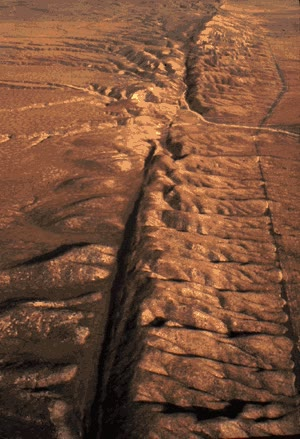
\includegraphics[width=0.28\linewidth]{images/book1/g7-usgs-san-andreas.jpg}

{\small The San Andreas fault crossing the Carrizo \omterm{def:g1:landscapes-around-us:landform}{Plain}, California, seen
from an aeroplane: the long straight \omterm{def:g1:landscapes-around-us:landform}{valley} is the boundary between the
Pacific \omterm{def:g7:plate-tectonics:plate}{plate} (left) and the North American \omterm{def:g7:plate-tectonics:plate}{plate} (right). Photograph:
Robert E. Wallace, U.S. Geological Survey (public domain).}
\end{omfigure}

\begin{method}[Recognising a plate boundary on a map]\label{met:g7:plate-tectonics:recognise}
To decide what kind of boundary separates two \omterm{def:g7:plate-tectonics:plate}{plates}:
\begin{enumerate}
  \item find, on a \omterm{def:g2:drawing-to-map:map}{map} of \omterm{def:g7:plate-tectonics:plate}{plate} motions, the arrows on either side of the
        boundary;
  \item if they point away from the boundary, it is divergent; if they
        point towards it, convergent; if they are parallel to it and point
        in opposite directions, transform;
  \item check with the \omterm{def:g1:landscapes-around-us:landscape}{landscape}: a ridge in the middle of an \omterm{def:g2:water-on-earth:ocean}{ocean} or a
        rift across a \omterm{def:g3:continents-and-oceans:continent}{continent} goes with a \omterm{def:g7:plate-tectonics:plate-boundary}{divergent boundary}; a deep
        trench with a line of \omterm{def:g4:volcanoes-earthquakes-first-look:volcano}{volcanoes}, or a high \omterm{def:g4:world-physical-map:range}{mountain range}, with a
        convergent one; a long straight fault with neither, with a
        \omterm{def:g7:plate-tectonics:plate-boundary}{transform boundary}.
\end{enumerate}
\end{method}

\section{How fast do plates move?}

\begin{proposition}[A few centimetres a year]\label{prop:g7:plate-tectonics:speed}
% ledger: data:pb2002 (speeds computed in figdata/grade-7/plate_speeds.py), usgs:mar-rate
Two neighbouring \omterm{def:g7:plate-tectonics:plate}{plates} move relative to each other at a speed of a few
centimetres per year: from about 2 centimetres per year across the
North Atlantic to more than 14 centimetres per year across the East Pacific
Rise, the fastest-spreading ridge on Earth.
\end{proposition}

\begin{omfigure}
\begin{tikzpicture}
\begin{axis}[xbar, width=0.82\linewidth, height=5.4cm, xmin=0, xmax=16.5,
  ytick={1,...,6}, yticklabels={North Atlantic ridge, South Atlantic ridge,
  San Andreas fault, Himalaya, Peru--Chile trench, East Pacific Rise},
  y tick label style={font=\small}, tick label style={font=\small},
  xlabel={speed of one plate relative to the other (cm per year)},
  label style={font=\small}, bar width=7pt, axis x line=bottom,
  axis y line=left, axis line style={-}, enlarge y limits=0.12,
  nodes near coords, nodes near coords style={font=\scriptsize},
  every node near coord/.append style={/pgf/number format/fixed,
  /pgf/number format/precision=1, /pgf/number format/fixed zerofill}]
\addplot[fill=omDef!55, draw=omDef!80!black] table[x=speed_cm_a, y=rank] {figdata/out/grade-7-plate_speeds.dat};
\end{axis}
\end{tikzpicture}

{\small How fast \omterm{def:g7:plate-tectonics:plate}{plates} move at six boundaries: averages along each boundary
computed from P.~Bird's \omterm{def:g7:plate-tectonics:plate}{plate} model (2003).}
\end{omfigure}

\begin{method}[From centimetres per year to kilometres per million years]\label{met:g7:plate-tectonics:convert}
A kilometre is \num{100000} centimetres. A speed of \qty{1}{cm} per year,
kept up for a million years, therefore covers \num{1000000} centimetres,
that is \qty{10}{km}. Hence:
\[
  1\ \text{cm per year} = 10\ \text{km per million years}.
\]
Multiply a speed in centimetres per year by 10 to get kilometres per
million years; then multiply by a number of millions of years to get a
distance in kilometres, or divide a distance by the speed to get a time.
\end{method}

\begin{example}[The Atlantic grows]\label{ex:g7:plate-tectonics:atlantic}
% ledger: usgs:mar-rate
On average, the two sides of the Mid-Atlantic Ridge move apart at about
\qty{2.5}{cm} per year, that is \qty{25}{km} per million years. In 100
million years that makes \qty{2500}{km}: kept up long enough, a speed far
too slow to notice in a lifetime opens an \omterm{def:g2:water-on-earth:ocean}{ocean}.
\end{example}

\begin{remark}[Measuring the motion today]\label{rem:g7:plate-tectonics:gps}
% ledger: usgs:gps
Such slow motions are now measured directly. Permanent stations fixed to
the \omterm{def:g3:stones-pebbles-sand:rock}{bedrock} receive the signals of positioning satellites and work out
their own position, day after day, to a few millimetres. Over a few years,
stations on different \omterm{def:g7:plate-tectonics:plate}{plates} are seen to move apart or closer together,
at the speeds found from the \omterm{def:g3:stones-pebbles-sand:rock}{rocks} over millions of years. Satellite
positioning itself is the subject of \cref{ch:g9:maps-of-the-earth}.
\end{remark}

\begin{omfigure}
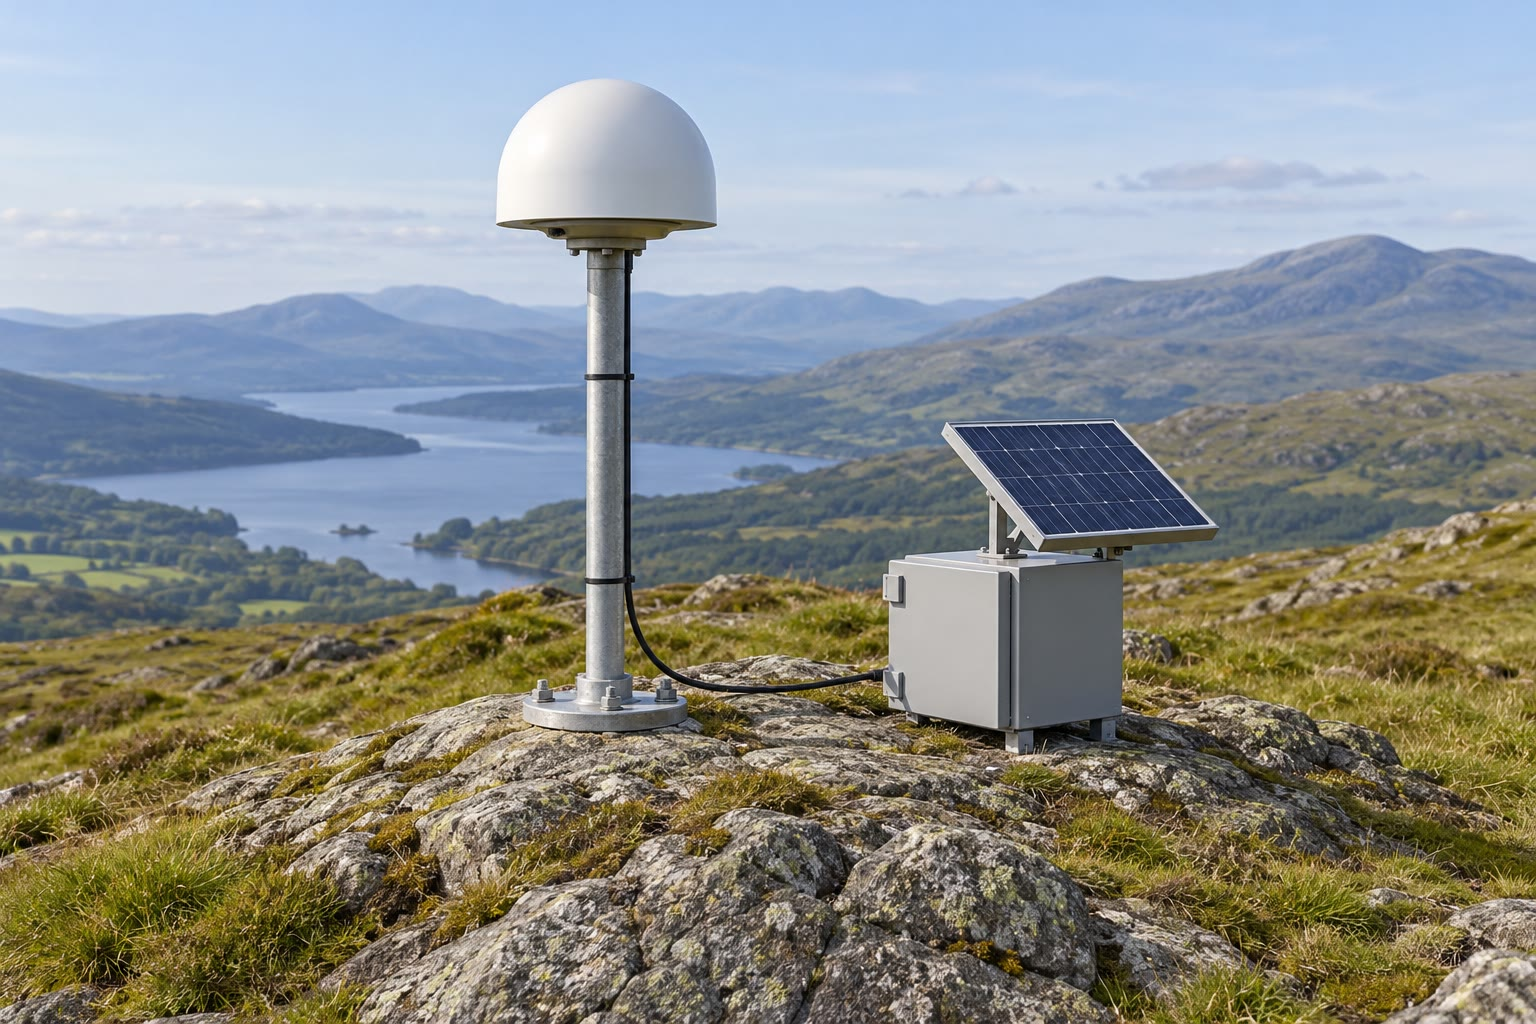
\includegraphics[width=0.55\linewidth]{images/book1/ai/g7-gps-station.jpg}

{\small A permanent positioning station: its antenna is bolted to the
\omterm{def:g3:stones-pebbles-sand:rock}{rock}, so it moves with the \omterm{def:g7:plate-tectonics:plate}{plate}.}
\end{omfigure}

\section{Exercises}

\begin{exercise}[$\star$]\label{exo:g7:plate-tectonics:1}
What is \omterm{def:g7:plate-tectonics:continental-drift}{continental drift}? Give the four kinds of clues Wegener used to
defend it.
\end{exercise}

\begin{exercise}[$\star$]\label{exo:g7:plate-tectonics:2}
Name the three kinds of \omterm{def:g7:plate-tectonics:plate-boundary}{plate boundary} and say, for each, how the two
\omterm{def:g7:plate-tectonics:plate}{plates} move with respect to each other.
\end{exercise}

\begin{exercise}[$\star$]\label{exo:g7:plate-tectonics:3}
Look at the \omterm{def:g2:drawing-to-map:map}{map} of \omterm{def:g4:volcanoes-earthquakes-first-look:earthquake}{earthquakes} and \omterm{def:g4:volcanoes-earthquakes-first-look:volcano}{volcanoes}. Name two regions of the
world with many large \omterm{def:g4:volcanoes-earthquakes-first-look:earthquake}{earthquakes}, and one \omterm{def:g3:continents-and-oceans:continent}{continent} that has almost
none in its middle.
\end{exercise}

\begin{exercise}[$\star$]\label{exo:g7:plate-tectonics:4}
Fossils of \emph{Mesosaurus}, a small reptile that lived in \omterm{def:g2:water-on-earth:salt-fresh}{fresh water},
are found in Brazil and in southern Africa. Why is this a clue that the two
\omterm{def:g3:continents-and-oceans:continent}{continents} were once joined?
\end{exercise}

\begin{exercise}[$\star\star$]\label{exo:g7:plate-tectonics:5}
Coal is found in Antarctica. What does this tell us about the \omterm{def:g5:weather-and-climate:climate}{climate} in
which the coal formed, and what can we conclude about where Antarctica was
at that time?
\end{exercise}

\begin{exercise}[$\star\star$]\label{exo:g7:plate-tectonics:6}
Say which kind of boundary is found at each of these places: the
Mid-Atlantic Ridge; the Andes; the San Andreas fault; the Himalaya; the
East African Rift.
\end{exercise}

\begin{exercise}[$\star\star$]\label{exo:g7:plate-tectonics:7}
Convert a speed of \qty{2.5}{cm} per year into kilometres per million
years. How far apart would two points on either side of the boundary move
in 60 million years at this speed?
\end{exercise}

\begin{exercise}[$\star\star$]\label{exo:g7:plate-tectonics:8}
Between 1975 and 1984 --- nine years --- the cracks near the Krafla \omterm{def:g4:volcanoes-earthquakes-first-look:volcano}{volcano}
in Iceland widened by about \qty{7}{m} in all. What was the average
widening per year, in centimetres? Compare it with the average speed of
the Mid-Atlantic Ridge, about \qty{2.5}{cm} per year, and suggest why the
two numbers are so different.
\end{exercise}

\begin{exercise}[$\star\star$]\label{exo:g7:plate-tectonics:9}
Wegener's theory was rejected for decades. What question could he not
answer? What does the theory of \omterm{def:g7:plate-tectonics:plate-tectonics}{plate tectonics} change in his picture of
moving \omterm{def:g3:continents-and-oceans:continent}{continents}?
\end{exercise}

\begin{exercise}[$\star\star$]\label{exo:g7:plate-tectonics:10}
Look at the cut through two \omterm{def:g7:plate-tectonics:plate-boundary}{plate boundaries}. Where is the \omterm{def:g2:water-on-earth:ocean}{sea} floor
highest, and where is it deepest? Where is new \omterm{def:g7:plate-tectonics:plate}{plate} being made, and where
does a \omterm{def:g7:plate-tectonics:plate}{plate} go back into the \omterm{def:g6:inside-the-earth:layers}{mantle}?
\end{exercise}

\begin{exercise}[$\star\star\star$]\label{exo:g7:plate-tectonics:11}
Across the East Pacific Rise the \omterm{def:g7:plate-tectonics:plate}{plates} move apart at about \qty{14.2}{cm}
per year, and across the North Atlantic ridge at about \qty{2.2}{cm} per
year. How many times faster is the East Pacific Rise (round to the nearest
whole number)? How long does each ridge take to open \qty{1000}{km} of new
\omterm{def:g2:water-on-earth:ocean}{ocean} floor?
\end{exercise}

\begin{exercise}[$\star\star\star$]\label{exo:g7:plate-tectonics:12}
% ledger: data:usgs-comcat, data:pb2002 (counts in figdata/grade-7/quakes_on_boundaries.py, part bands)
Of the 7\,031 \omterm{def:g4:volcanoes-earthquakes-first-look:earthquake}{earthquakes} of magnitude 6 or more recorded from 1976 to
2025, 4\,578 happened less than \qty{100}{km} from the line of a \omterm{def:g7:plate-tectonics:plate-boundary}{plate
boundary} drawn on the \omterm{def:g2:drawing-to-map:map}{map}, 6\,472 less than \qty{300}{km} and 6\,786 less
than \qty{500}{km}.
(a) How many happened between \qty{100}{km} and \qty{300}{km} from the
line? (b) Work out, to the nearest whole number, the percentage of all
these \omterm{def:g4:volcanoes-earthquakes-first-look:earthquake}{earthquakes} that happened less than \qty{100}{km} from the line.
(c) Many of the \omterm{def:g4:volcanoes-earthquakes-first-look:earthquake}{earthquakes} between \qty{100}{km} and \qty{300}{km} from
the line lie on the same side of a deep \omterm{def:g2:water-on-earth:ocean}{ocean} trench. Using what happens
at a \omterm{def:g7:plate-tectonics:plate-boundary}{convergent boundary}, explain why an \omterm{def:g4:volcanoes-earthquakes-first-look:earthquake}{earthquake} caused by a \omterm{def:g7:plate-tectonics:plate-boundary}{plate
boundary} can happen so far from the line drawn on the \omterm{def:g2:drawing-to-map:map}{map}.
\end{exercise}

\section{Problem: Opening the South Atlantic}

\begin{problem}[{Weekend problem --- measuring an ocean on the map and
finding how long it took to open}]
\label{pb:g7:plate-tectonics:1}
% ledger: data:ne-land, earth:Rmean, data:pb2002, usgs:pangaea-breakup, usgs:atlantic-growth
% (all numbers computed in figdata/grade-7/south_atlantic.py: coasts at 23 S
% at 43.21 W and 14.39 E, 102.4 km per degree, AF-SA full rate 3.43 cm/yr)
On a \omterm{def:g2:drawing-to-map:map}{map} of the South Atlantic, a student follows the \omterm{def:g6:latitude-longitude:latitude}{parallel} at
\omterm{def:g6:latitude-longitude:latitude}{latitude} \ang{23} South. It leaves the \omterm{def:g1:landscapes-around-us:water}{coast} of South America near Rio de
Janeiro, at \omterm{def:g6:latitude-longitude:longitude}{longitude} \ang{43.2} West, crosses the \omterm{def:g2:water-on-earth:ocean}{ocean} and the
Mid-Atlantic Ridge, and reaches the \omterm{def:g1:landscapes-around-us:water}{coast} of Africa near Walvis Bay, at
\omterm{def:g6:latitude-longitude:longitude}{longitude} \ang{14.4} East. On this \omterm{def:g6:latitude-longitude:latitude}{parallel}, one degree of \omterm{def:g6:latitude-longitude:longitude}{longitude}
measures \qty{102}{km}. Across the ridge, at this \omterm{def:g6:latitude-longitude:latitude}{latitude}, the South
American and African \omterm{def:g7:plate-tectonics:plate}{plates} move apart at \qty{3.4}{cm} per year.

\begin{center}
\begin{tikzpicture}
\begin{axis}[axis equal image, xmin=-60, xmax=30, ymin=-42, ymax=12,
  width=0.6\linewidth, tick label style={font=\scriptsize},
  xtick={-60,-40,...,20}, ytick={-40,-20,0},
  xticklabel={$\pgfmathprintnumber{\tick}^\circ$},
  yticklabel={$\pgfmathprintnumber{\tick}^\circ$},
  axis background/.style={fill=omSea}]
\addplot[fill=omLithAlluv, draw=black!45, line width=0.3pt] table {figdata/out/shared-geo-land.dat};
\addplot[omRidge, line width=0.9pt, unbounded coords=jump, restrict x to domain=-45:5] table {figdata/out/shared-geo-school-ridge.dat};
\addplot[omRidge!70!black, line width=0.9pt, unbounded coords=jump, restrict x to domain=-45:5] table {figdata/out/shared-geo-school-transform.dat};
\draw[black, densely dashed, line width=0.7pt] (axis cs:-43.21,-23) -- (axis cs:14.39,-23);
\fill (axis cs:-43.21,-23) circle (1.5pt);
\fill (axis cs:14.39,-23) circle (1.5pt);
\node[font=\scriptsize, below right, inner sep=2pt] at (axis cs:-43.21,-23) {Rio de Janeiro};
\node[font=\scriptsize, below left, inner sep=2pt] at (axis cs:14.39,-23) {Walvis Bay};
\node[font=\scriptsize, anchor=east, inner sep=1pt] at (axis cs:-16.5,-34) {Mid-Atlantic Ridge};
\end{axis}
\end{tikzpicture}
\end{center}

\medskip
\noindent\textbf{Part I --- The clues of the fit.}
\begin{enumerate}
  \item On the fossil \omterm{def:g2:drawing-to-map:map}{map} of this chapter, name the fossils whose bands
        cross from South America into Africa.
  \item Why can the fossils of \emph{Mesosaurus} not be explained by an
        animal that swam from one \omterm{def:g3:continents-and-oceans:continent}{continent} to the other?
  \item Which part of South America fits into which part of Africa?
  \item What kind of \omterm{def:g7:plate-tectonics:plate-boundary}{plate boundary} runs down the middle of the South
        Atlantic today? How do the two \omterm{def:g7:plate-tectonics:plate}{plates} move there?
\end{enumerate}

\medskip
\noindent\textbf{Part II --- Measuring the ocean.}
\begin{enumerate}[resume]
  \item How many degrees of \omterm{def:g6:latitude-longitude:longitude}{longitude} separate the two \omterm{def:g1:landscapes-around-us:water}{coasts} along the
        \omterm{def:g6:latitude-longitude:latitude}{parallel} at \ang{23} South?
  \item What is the width of the \omterm{def:g2:water-on-earth:ocean}{ocean}, in kilometres, along this
        \omterm{def:g6:latitude-longitude:latitude}{parallel}? Round to the nearest ten kilometres.
  \item At the \omterm{def:g3:continents-and-oceans:equator}{equator}, one degree of \omterm{def:g6:latitude-longitude:longitude}{longitude} measures \qty{111}{km}.
        Why is it only \qty{102}{km} at \ang{23} South?
  \item The ridge runs roughly down the middle of the \omterm{def:g2:water-on-earth:ocean}{ocean}. About how far
        from the ridge is each \omterm{def:g1:landscapes-around-us:water}{coast}?
\end{enumerate}

\medskip
\noindent\textbf{Part III --- The age of the ocean.}
\begin{enumerate}[resume]
  \item Convert the speed at which the two \omterm{def:g7:plate-tectonics:plate}{plates} move apart into
        kilometres per million years.
  \item If the \omterm{def:g2:water-on-earth:ocean}{ocean} had always opened at this speed, how many million
        years would it have taken to reach its present width? Round to
        the nearest ten million years.
  \item Geologists date the break-up of \omterm{def:g7:plate-tectonics:supercontinent}{Pangaea} at between about 225 and
        200 million years ago, and say that the Atlantic has grown over the
        last 100 to 200 million years. Does your answer agree with this?
  \item Give one reason why the true age of the South Atlantic may differ
        from the age you found.
\end{enumerate}
\end{problem}
